\begin{center}
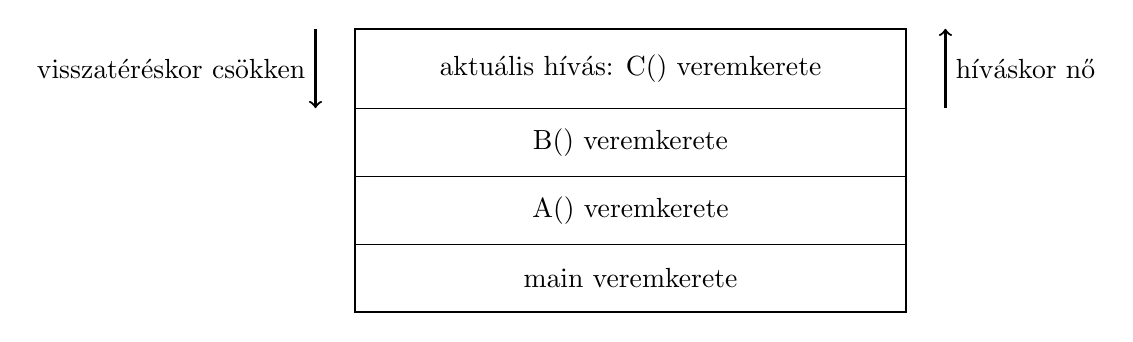
\begin{tikzpicture}[x=1cm,y=0.72cm]
  \draw[thick] (0,0) rectangle (7,5);
  \draw (0,1.2) -- (7,1.2);
  \draw (0,2.4) -- (7,2.4);
  \draw (0,3.6) -- (7,3.6);
  \node at (3.5,0.6) {main veremkerete};
  \node at (3.5,1.8) {A() veremkerete};
  \node at (3.5,3.0) {B() veremkerete};
  \node at (3.5,4.3) {aktuális hívás: C() veremkerete};
  \draw[->, thick] (7.5,3.6) -- (7.5,5.0) node[midway,right] {híváskor nő};
  \draw[->, thick] (-0.5,5.0) -- (-0.5,3.6) node[midway,left] {visszatéréskor csökken};
\end{tikzpicture}
\end{center}
